\section{Devices}

\begin{frame}{Device connections} Devices, with connections, used in our
research: \vspace{0.5cm}

\begin{columns}[T] \column{0.33\textwidth} \centering \textbf{Burlington}
  \begin{figure}[h] \centering
    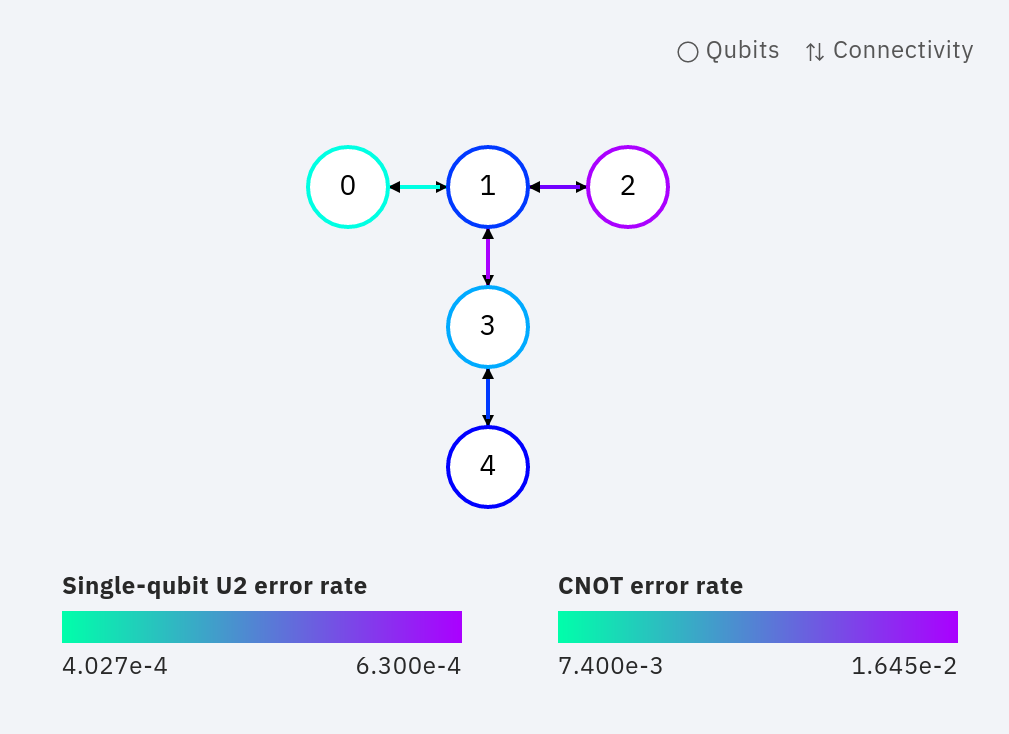
\includegraphics[width=\textwidth]{images/connection_diagram_burlington.png}
    \label{fig:burlington_connections}
  \end{figure}

  \column{0.33\textwidth} \centering \textbf{Melbourne}
  \begin{figure}[h] \centering
    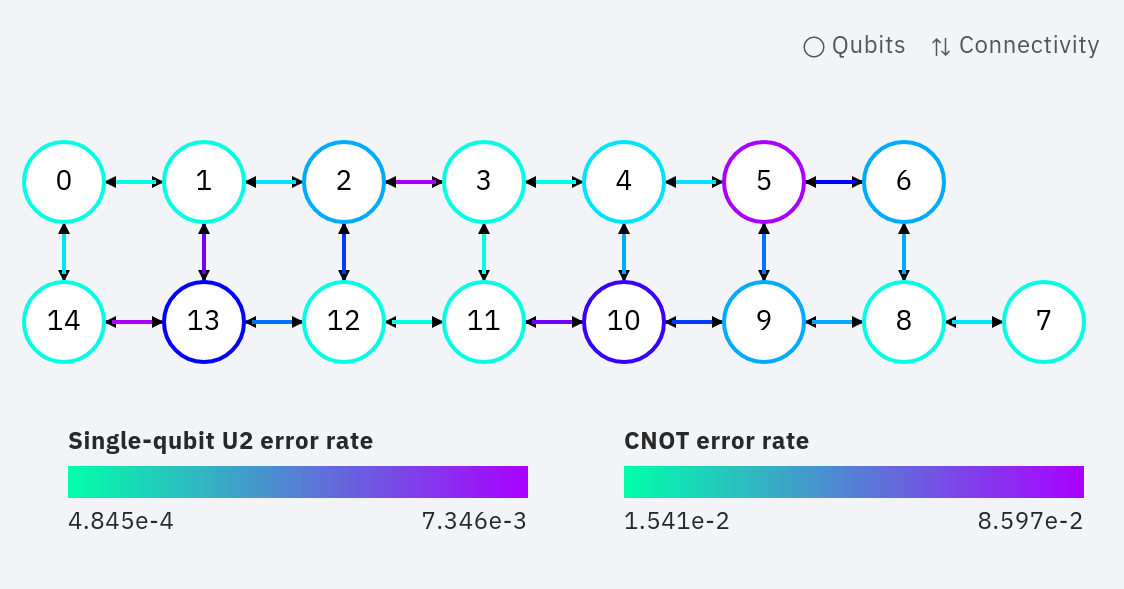
\includegraphics[width=\textwidth]{images/connection_diagram_melbourne.png}
    \caption*{\tiny Only qubits 0, 1, 2 and 14 were used.}
    \label{fig:melbourne_connections}
  \end{figure}

  \column{0.33\textwidth} \centering \textbf{Yorktown}
  \begin{figure}[h] \centering
    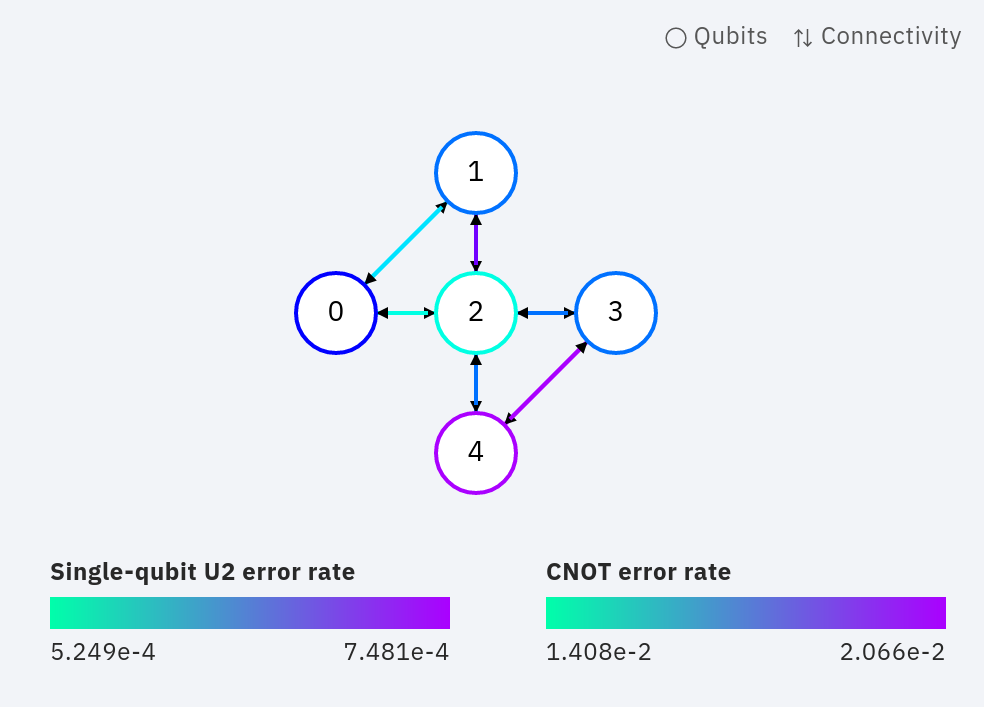
\includegraphics[width=\textwidth]{images/connection_diagram_ibmqx2.png}
    \label{fig:ibmqx2_connections}
  \end{figure}

\end{columns}
  Device connections have a significant impact on the number of gates required
to run a circuit.
\end{frame}

\begin{frame}{Example: Yorktown versus Burlington}
Yorktown and Burlington both 5 qubit devices, but give different number of
required gates (for Purification protocol)

\begin{figure}[h] \centering
	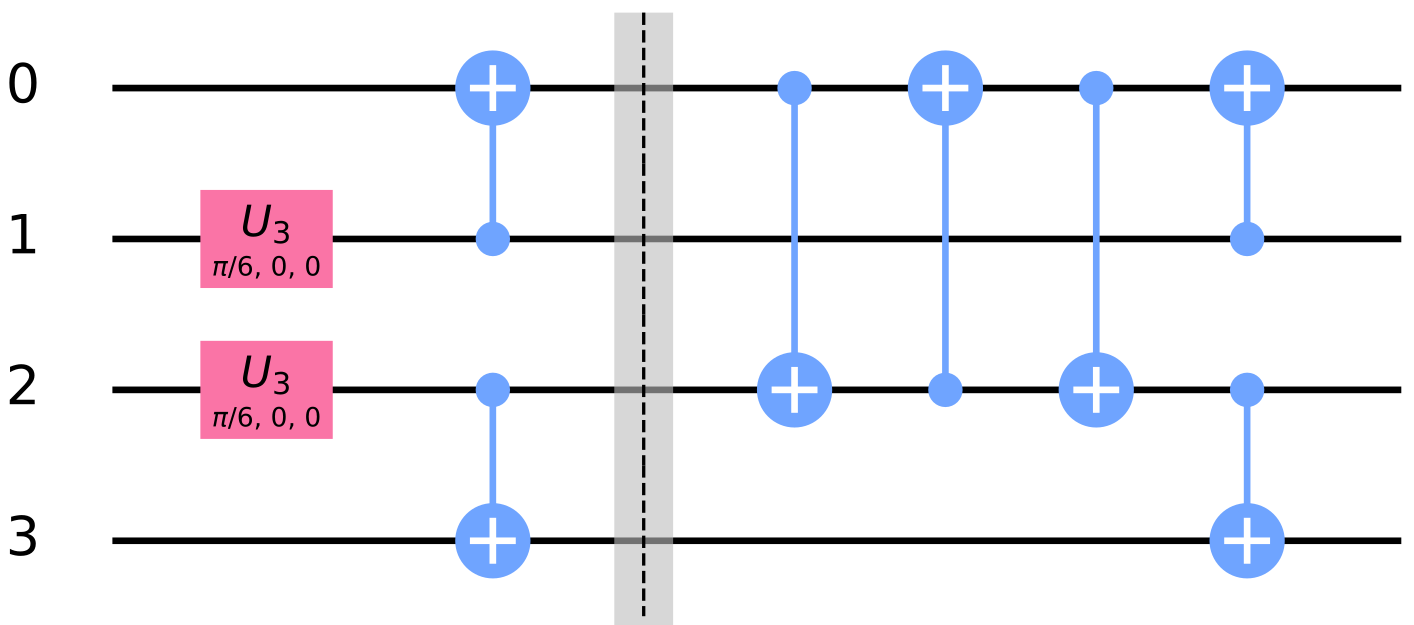
\includegraphics[width=0.5\textwidth]{images/purification_ibmqx2.png}
	\caption*{\tiny Yorktown (7 CNOT gates)}
	\label{fig:pure_york}
\end{figure}

\begin{figure}[h] \centering
	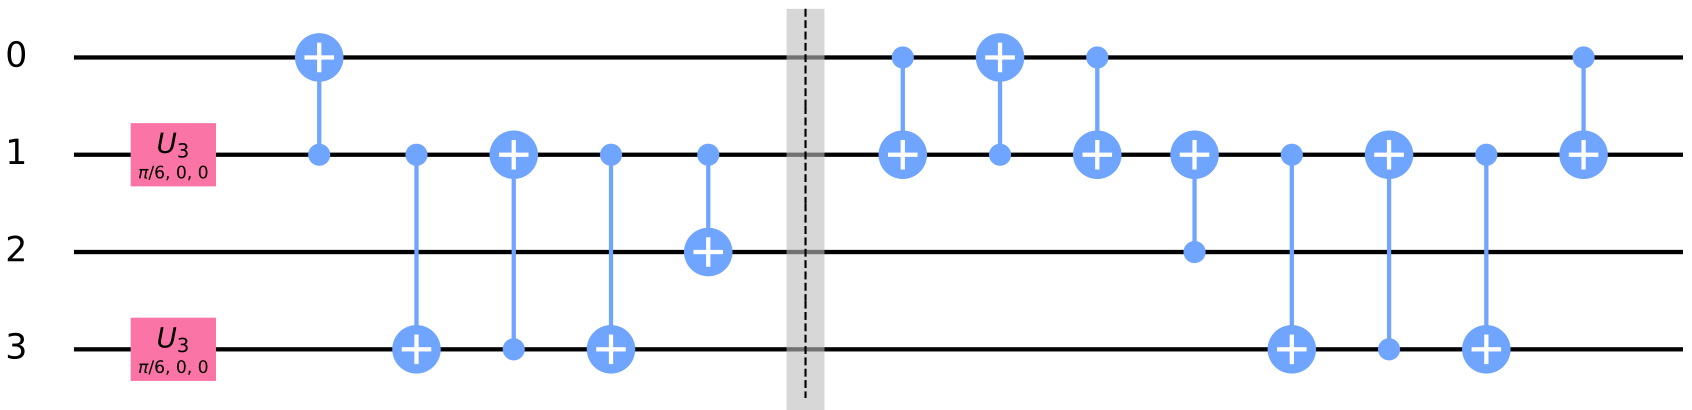
\includegraphics[width=0.8\textwidth]{images/purification_burlington.png}
	\caption*{\tiny Burlington (13 CNOT gates)}
	\label{fig:pure_burl}
\end{figure}
\end{frame}

\begin{frame}{Error percentage}
Average percent error on single qubit $U_2$ and CNOT gates.
\vspace{0.5cm}
\begin{table} \centering
	\begin{tabular}{lrrrr} \toprule Backend & $U_2 (\%)$ & $CNOT (\%)$ \\ \midrule
		Burlington & 0.050 & 1.213 \\ Melbourne & 1.258 & 2.156 \\ Yorktown & 0.689 &
		2.275 \\ \bottomrule
	\end{tabular}
	\label{tb:average_errors}
\end{table}
\vspace{0.5cm}
\begin{itemize}
  \item Burlington has lowest average error, but this doesn't necessarily mean
better fidelity, as the number of gates for each circuit varies per device.
  \item Yorktown, with highest average CNOT fidelity, still often outperforms other
backends.
\end{itemize}
\end{frame}

\section{Quantum Circuits}

\begin{frame}{The Teleportation protocol}
	
	\begin{block}{Circuit run}
		\begin{itemize}
			\item Initialize random state on first qubit.
			\item Initialize $\ket{\Phi^+}$ Bell state on bottom qubits.
			\item CNOT gate on qubit 0 and 1.
			\item Hadamard gate on qubit 0.
		\end{itemize}
	\end{block}
	
	\begin{figure}[h] \centering
		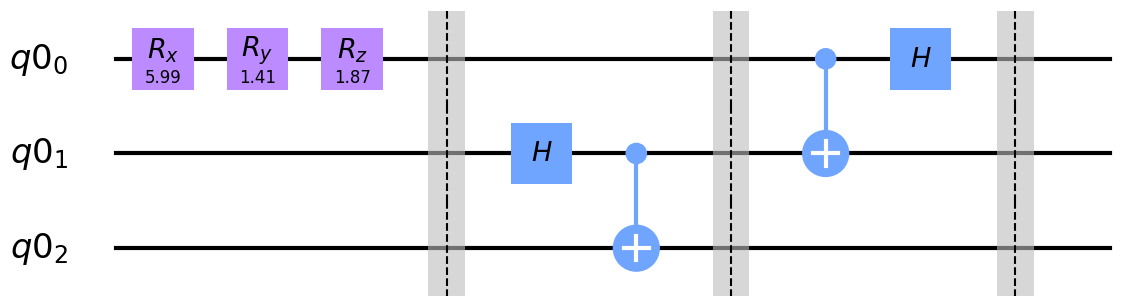
\includegraphics[width=\textwidth]{images/teleport_circuit.png}
		\label{fig:tele_circ}
	\end{figure}

\end{frame}

\begin{frame}{The Teleportation protocol}

No operations possible after measurement on IBM Q devices. So, resort to post
measurement techniques. If measurement of qubit 0 and 1 gives -1, Pauli-Z and
Pauli-X matrix are applied, respectively.
\vspace{0.5cm}
\begin{figure}[h] \centering
  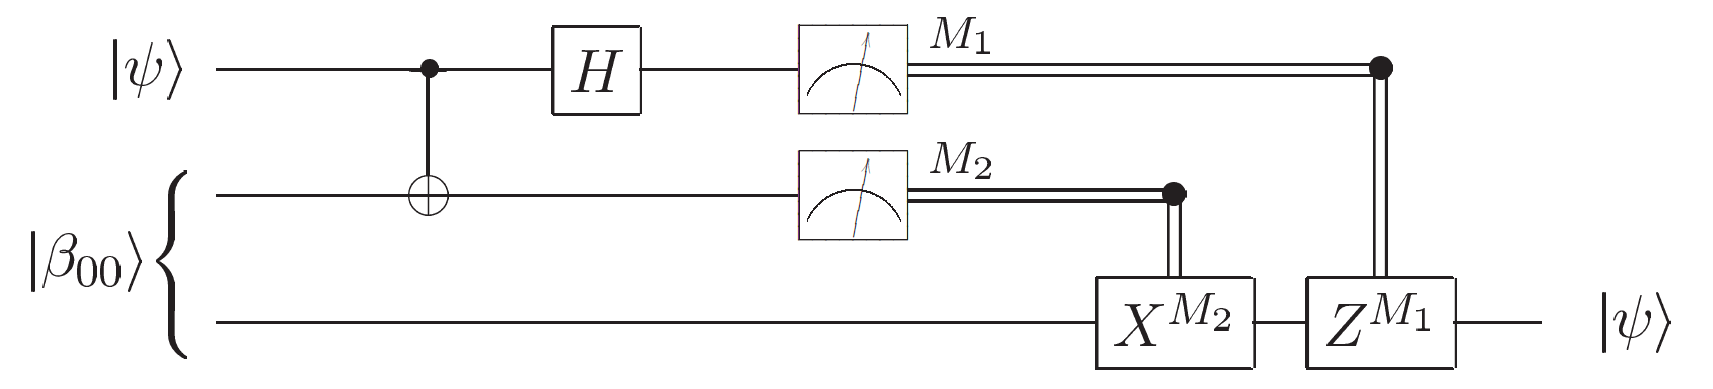
\includegraphics[width=\textwidth]{images/Teleport_general.png}
  \label{fig:tele_gen}
\end{figure}
	
\end{frame}

\begin{frame}{Entanglement swap}
	
\begin{block}{Circuit run}
  \begin{itemize}
    \item Initialize random Bell-like state on top qubits.
    \item Initialize $\ket{\Phi^+}$ Bell state on bottom qubits.
    \item CNOT gate on qubit 1 and 2.
    \item Hadamard gate on qubit 1.
  \end{itemize}
\end{block}

\begin{figure}[h] \centering
  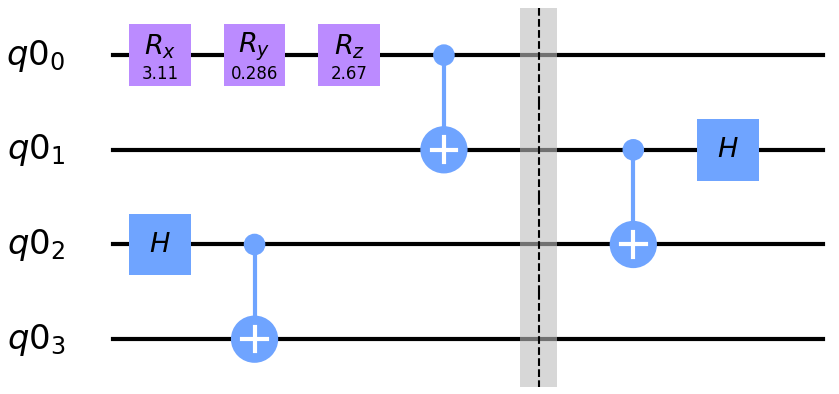
\includegraphics[width=0.8\textwidth]{images/swap_circuit.png}
  \label{fig:swap_circ}
\end{figure}
	
\end{frame}

\begin{frame}{Entanglement swap}
Again, resort to post measurement techniques. If measurement of qubit 1 and 2
gives -1, Pauli-Z and Pauli-X matrix are applied, respectively. This creates
entanglement between qubits 0 and 3 of the random Bell-like state.
\vspace{0.5cm}
  \begin{figure}[h] \centering
  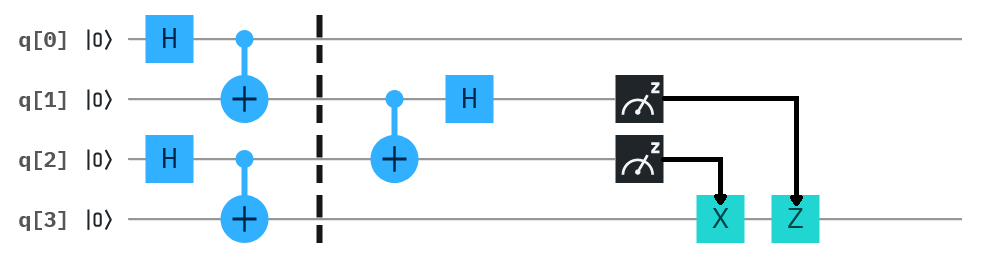
\includegraphics[width=0.8\textwidth]{images/swap_general.png}
  \label{fig:swap_gen}
\end{figure}
	
\end{frame}

\begin{frame}{Entanglement purification}
	
\begin{block}{Circuit run}
  \begin{itemize}
    \item Initialize two Bell-like state on top and bottom qubits by rotating
$\theta = \arcsin{\left(2F-1\right)}$. Where $F$ is the input fidelity.
    \item CNOT gate on qubit 1 and 3.
    \item CNOT gate on qubit 2 and 4.
  \end{itemize}
\end{block}
	
\begin{figure}[h] \centering
  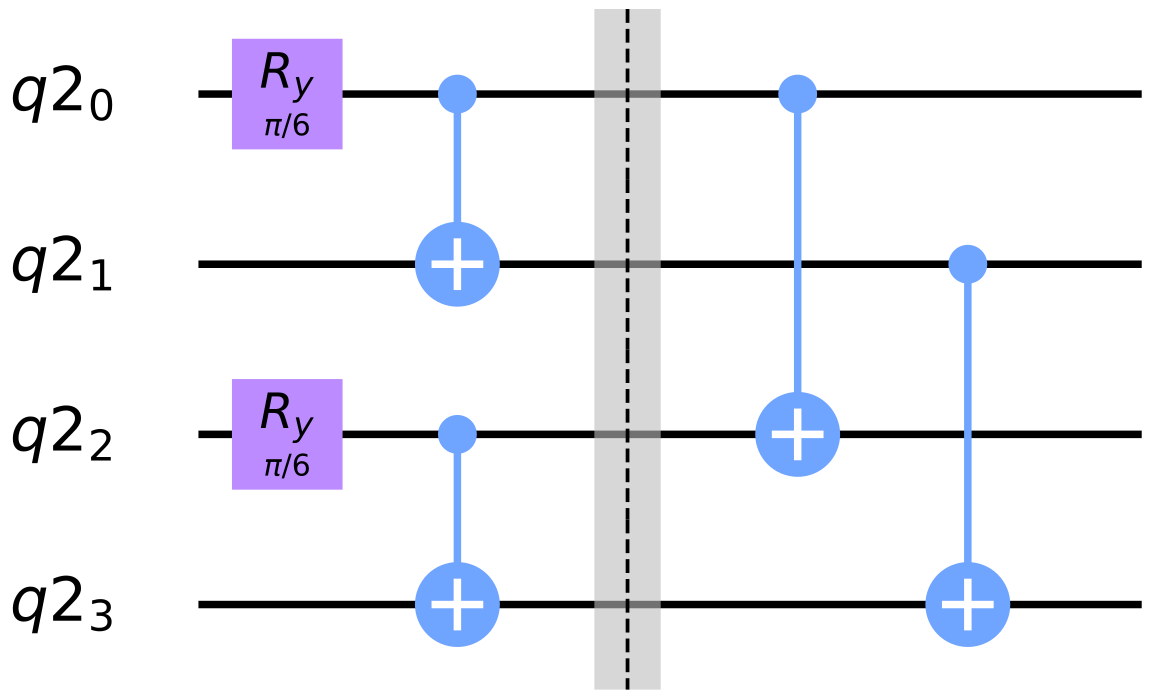
\includegraphics[width=0.6\textwidth]{images/purification_circuit.png}
  \label{fig:puri_circ}
\end{figure}
	
\end{frame}

\begin{frame}{Entanglement purification}
	
\begin{block}{Circuit run (with states)}
  \begin{itemize}
    \item $\ket{\Psi} = 0.933\ket{0000}+0.067\ket{1111}
    +0.250\left(\ket{0011}+\ket{1100}\right)$
    \item $\ket{\Psi} = 0.933\ket{0000}+0.067\ket{1011}
    +0.250\left(\ket{0111}+\ket{1100}\right)$
    \item $\ket{\Psi} =
    0.933\ket{0000}+0.067\ket{0011} +0.250\left(\ket{1111}+\ket{1100}\right)$
  \end{itemize}
\end{block}

Measuring bottom two qubits in $\ket{11}$ (which occurs with a probability of
$12.5\%$) gives the top two qubit state $\ket{\Psi_{1,2}} =
\frac{1}{\sqrt{2}}\left(\ket{11} +\ket{00}\right) = \ket{\Phi^+}$ .
	
\begin{figure}[h] \centering
  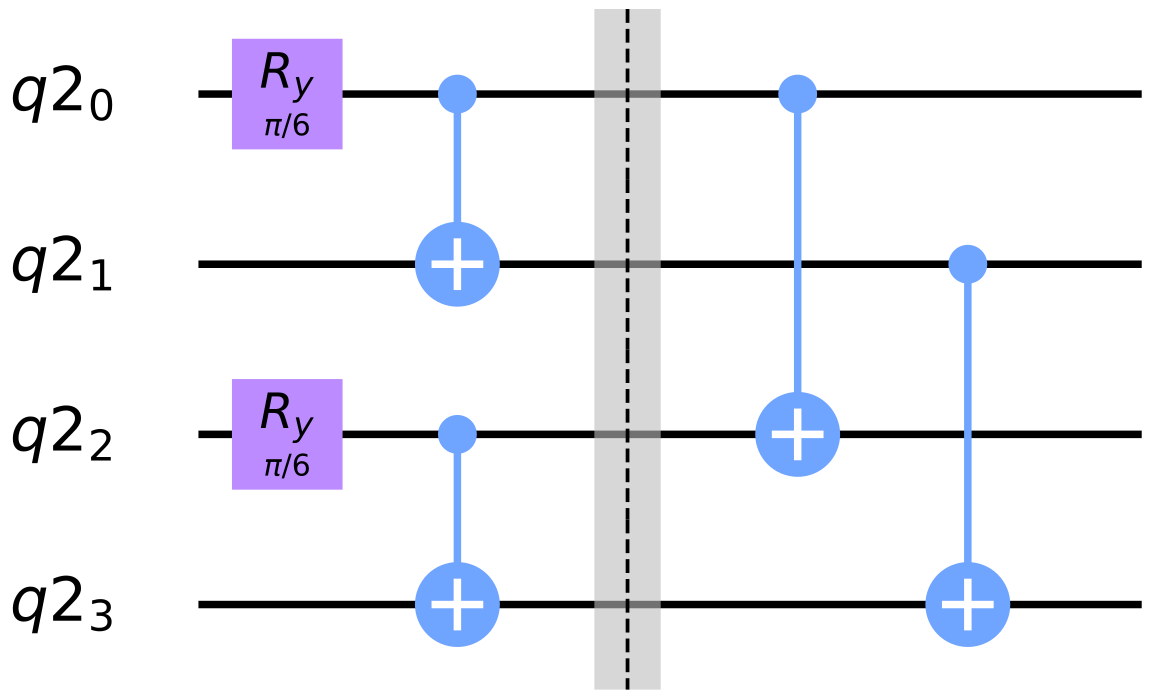
\includegraphics[width=0.5\textwidth]{images/purification_circuit.png}
  \label{fig:puri_circ}
\end{figure}
	
\end{frame}

\begin{frame}{Grover's search algorithm}
		
\begin{block}{Circuit run}
  \begin{itemize}
    \item Apply Hadamard gate to the two qubits.
    \item Apply diagonal matrix with three values of 1 and one -1 (rest of matrix is 0).
    \item Do an inversion about the mean.
  \end{itemize}
\end{block}


\begin{figure}[h] \centering
  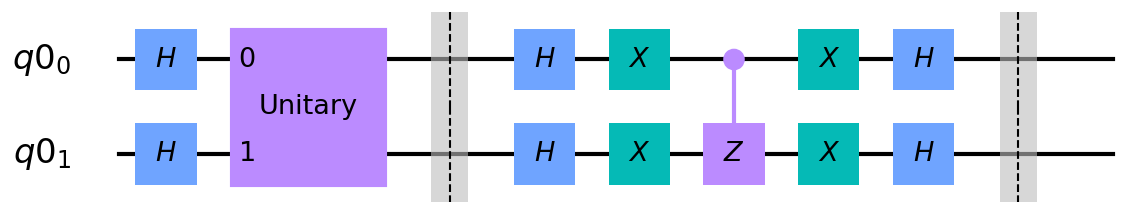
\includegraphics[width=\textwidth]{images/grover_circuit.png}
  \label{fig:grov_circ}
\end{figure}
Measurement of the circuit gives position of the -1 in the diagonal matrix. For
example, $\ket{11}$ measurement is the fourth position
	
\end{frame}

%%% Local Variables:
%%% mode: latex
%%% TeX-master: "presentation"
%%% End: